% Chapter 3

\chapter{Introduction to the Player Study}

\label{chapter:player-study-introduction}
\lhead{Chapter \ref{chapter:player-study-introduction}. \emph{Player Study - Introduction}}

% Section 1 - Survey distribution
\section{Survey Distribution}

The survey was distributed in a Norwegian and an English version, and in multiple phases. After the first phase, some questions were adjusted, and a missing question regarding weight loss and perceived improvement on physical health was added. The final version of the survey can be found in Appendix \ref{appendix:survey}.

The first phase of distribution took place at a large Pokémon Go event in \emph{Frognerparken} in Oslo, Norway, a large sculpture park and popular destination for Pokémon Go players due to the high density of Pokéstops and spawns. The survey was available online via an easily accessible custom URL from a known link shortener, leading to the Norwegian version. Single players and groups of players were approached over the span of about two hours, given a short introduction to the project and asked whether they would be willing to respond to the survey. Given a positive response, they were handed a note with the URL. Extra effort was made to reach out to players in the following categories: Young children (15 or below), parents playing with children, and players above 40. This was done in an attempt to reach the broad spectrum of ages participating, even though the bulk of players are between the ages of 20 and 35. \todo{Should I mention the number of responses that (likely) originated from here?}

In the second phase, the survey was distributed on \emph{Facebook}. A post explaining the project and an encouragement to respond despite the length of the survey, along with links to both versions, was shared in each of the four largest Norwegian Pokémon Go groups (\emph{Pokémon GO: Norway}, \emph{Pokemon Go Norge}, \emph{Pokémong GO - Oslo \& Akershus} and \emph{Pokémon GO Trondheim}), as well as personally. It was then re-shared by several people to their local Pokémon GO groups or their personal friends and followers. \todo{Could mention an estimate of the amount of people reached through these groups, and the amount of responses it yielded?}

The third phase involved sharing the survey on the popular internet forum \emph{Reddit}. Here it was shared in two \emph{subreddits}, sub-forums on the larger site with their own dedicated communities. The first subreddit was \emph{/r/PokemonGo}, the main community for people interested in the game in general. The second, \emph{/r/TheSilphRoad}, is a community devoted to research on all things related to Pokémon GO.

In addition to the three main phases of distribution, people encountered playing or talking about the game at any time were approached and asked to participate throughout all of September.

In early December, the respondents who had left contact information were contacted with a short follow-up survey, seen in Appendix \ref{appendix:followup}. Those who had left comments of note separating them from the other respondents were also asked about these points of interest. This second questionnaire was an attempt to gather information on the longevity of the game, some clarifications of questions from the original survey and a question about spending money in the game. 

\todo{Perhaps include a figure of the distribution of link clicks?}

% Section 2 - Demographics
\section{Demographics}

The survey collected data on the demographics of its respondents, including the age, gender and the country in which most of their playing occurred. The recorded nation is assumed to be their country of residence in most cases. A total of 2190 responses were recorded with demographic data.

Out of everyone who responded, 1244 (slightly below 57 \%) were male and 946 were female. Figure \ref{fig:respondents-age-histogram} shows a histogram of the ages of all respondents, ranging from 5 to 67 years old, with the largest number of respondents (176) being aged 25. Respondents have also been divided into seven different age groups, show in Table \ref{tbl:survey-age-distribution}. Note that the total percentages are rounded, and rounding errors cause the total to sum up to 101 \%.

\begin{figure}[h]
	\centering
	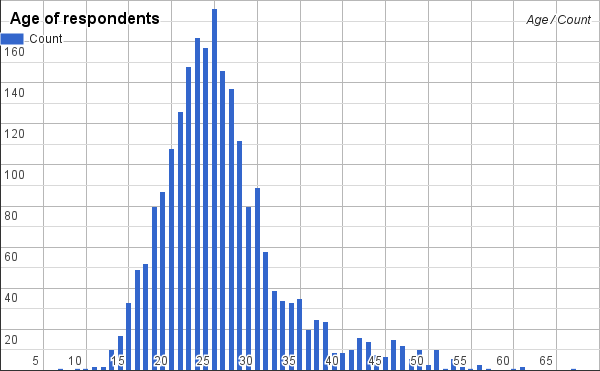
\includegraphics[width=\textwidth]{Figures/age-histogram}
	\caption{A histogram of the ages of the respondents}
	\label{fig:respondents-age-histogram}
\end{figure}

\begin{table}[h]
	\centering
	\caption{Age distribution of survey respondents}
	\label{tbl:survey-age-distribution}
	\begin{tabular}{|l||c|c|c|c|c|c|c|}
		\hline
		&\textbf{18-} & \textbf{18-21} & \textbf{22-26} & \textbf{27-32} & \textbf{33-40} & \textbf{41-50} & \textbf{50+}\\
		\hline\hline
		
		\textbf{Male} & 120 & 247 & 434 & 284 & 108 & 37 & 14 \\
		\hline
		
		\textbf{Female} & 48 & 154 & 355 & 231 & 81 & 64 & 14 \\
		\hline
		
		\textbf{Total} & 168 & 401 & 789 & 515 & 189 & 101 & 28 \\
						& 8\% & 18\% & 36\% & 24\% & 9\% & 5\% & 1\%\\
		\hline
	\end{tabular}
\end{table}

\todo{Mention the results normalized for responses per gender: More popular among males in the younger categories and females in the older categories (even in the middle). Matches observations of groups of young boys playing but few young girls, and maybe a reference to older women and walking groups}

The results contained 1192 responses stating Norway as their main location for playing. Because the survey was distributed in Norwegian Facebook groups, but not in local communities for other countries, Norway has been excluded from the following \todo{table/figure}, which shows the distribution of players per country for the remaining 998 respondents.

\todo{Include table or figure showing the countries of respondents}

The survey also asked for the main occupation of each respondent, with four categories available: employed, unemployed, higher education (e.g. university or college) and lower education (e.g. high school or middle school). The following table again shows the distribution between these categories. \todo{This data probably isn't very relevant and could possibly be removed.}

\begin{table}[h]
	\centering
	\caption{Distribution of survey respondents across occupations}
	\label{tbl:survey-occupation-distribution}
	\begin{tabularx}{\textwidth}{|l|l|X|X|}
		\hline
		\textbf{Lower education} & \textbf{Higher education} & \textbf{Employed} & \textbf{Unemployed}\\
		\hline\hline
		
		219 & 747 & 1056 & 169\\
		\hline
	\end{tabularx}
\end{table}

% Section 3 - Mapping to research questions
\section{Survey and Research Questions}

The purpose of the survey was to collect data to answer the research questions presented in Chapter \ref{chapter:research-questions}. This section will provide a mapping between the questions of the survey and the research questions each of them aim to answer. It should be noted that in addition to the listed questions, the survey included a comment section at the end where respondents could provide any additional info they did not find a proper place for, and these comments have also been used to evaluate the research questions.

\todo{Consider using tree graphs instead of tables to illustrate}

The first research goal, examining the success factors of Pokémon GO as seen in Section \ref{rg1}, was decomposed into five research questions, \ref{RQ1.1} through \ref{RQ1.5}. Table \ref{tbl:rg1-survey-questions} shows the survey questions relevant for this research goal and the research questions each of them help answering.

\begin{table}[h]
	\caption{\emph{What are the main factors that made Pokémon GO successful?} Survey Questions}
	\centering
	\label{tbl:rg1-survey-questions}
	\begin{tabularx}{\textwidth}{|X|l|}
		\hline
		\textbf{Survey question} & \textbf{Research questions}\\
		\hline\hline
		
		Which of the following factors influenced your decision to start playing Pokémon Go? & \ref{RQ1.1}\\
		\hline
		
		Which of the following game features do you use? & \ref{RQ1.2}\\
		\hline
		
		If you have previously played any location-based or augmented reality games, what did you like about them and what did you not like about them? How does Pokémon Go compare on these points? & \ref{RQ1.3}\\
		\hline
		
		If you have previously played any other casual mobile games, what did you like about them and what did you not like about them? How does Pokémon Go compare on these points? & \ref{RQ1.3}\\
		\hline
		
		If you have previously played any other Pokémon games, what did you like about them and what did you not like about them? How does Pokémon Go compare on these points? & \ref{RQ1.4}\\
		\hline
		
		If you are no longer playing, when and why did you stop? If you are still playing, but have greatly reduced the amount you play, when and why did this happen? & \ref{RQ1.5}\\
		\hline
	\end{tabularx}
\end{table}

The second research goal, evaluating the physical health effect of playing Pokémon GO as seen in section \ref{rg2} was decomposed into six research questions, \ref{rq-physical-activity-amount} through \ref{rq-physical-risks}. Table \ref{tbl:rg2-survey-questions} shows the survey questions relevant for this research goal and the research questions each of them help answering.

\begin{table}[h]
\caption{\emph{What are the effects on physical health from playing Pokémon GO, and how much effort does it take to achieve this effect?} Survey Questions}
\centering
\label{tbl:rg2-survey-questions}
	\begin{tabularx}{\textwidth}{|X|l|}
		\hline
		\textbf{Survey question} & \textbf{Research questions}\\
		\hline\hline
		
		In an average week, how much time did you spend on physical activities (e.g. walking, running or biking) before you started playing Pokémon Go? & \ref{rq-physical-activity-amount}, \ref{rq-physical-high-low-comparison}\\
		\hline
		
		In an average week, how much time do you spend on physical activities since you started playing Pokémon Go? & \ref{rq-physical-activity-amount}, \ref{rq-physical-high-low-comparison}\\
		\hline
		
		If you spend more time on physical activities after you started playing Pokémon Go than before, what are the sources of this activity? & \ref{rq-physical-game-activities}\\
		\hline
		
		Have you lost weight or in other ways feel more healthy than before you started playing Pokémon Go? & \ref{rq-physical-weight-loss}\\
		\hline
		
		Have you skipped out on less healthy activities (e.g. going out to drink) that you otherwise would have engaged in due to playing Pokémon Go instead? If so, please specify. & \ref{rq-physical-unhealthy-habits}\\
		\hline
		
		Have you trespassed or otherwise gone into areas you shouldn’t be because you were playing Pokémon Go? & \ref{rq-physical-risks}\\
		\hline
		
		Have you put yourself or others in dangerous situations because you were playing Pokémon Go? & \ref{rq-physical-risks}\\
		\hline
		
		Have you gotten into any accidents because either you or another involved party was playing Pokémon Go? & \ref{rq-physical-risks}\\
		\hline
		
		If you have put yourself or others in dangerous situations, or gotten into accidents, because of Pokémon Go, could you elaborate? & \ref{rq-physical-risks}\\
		\hline
		
		Have you neglected other areas of your life because you were playing Pokémon Go? & \ref{rq-physical-risks}\\
		\hline
	\end{tabularx}
\end{table}

The third research goal, evaluating the mental health effect of playing Pokémon GO as seen in section \ref{rg2} was decomposed into four research questions, \ref{rq-mental-social-activity-amount} through \ref{rq-mental-illnesses}. Table \ref{tbl:rg3-survey-questions} shows the survey questions relevant for this research goal and the research questions each of them help answering.

\begin{table}[h]
	\caption{\emph{What are the effects on mental health from playing Pokémon GO?} Survey Questions}
	\centering
	\label{tbl:rg3-survey-questions}
	\begin{tabularx}{\textwidth}{|X|l|}
		\hline
		\textbf{Survey question} & \textbf{Research questions}\\
		\hline\hline
		
		In an average week, during your spare time, how much time did you spend socializing with other people (in person, outside your home) before you started playing Pokémon Go? & \ref{rq-mental-social-activity-amount}\\
		\hline
		
		In an average week, during your spare time, how much time do you spend socializing with other people (in person, outside your home) since you started playing Pokémon Go? & \ref{rq-mental-social-activity-amount}\\
		\hline
		
		If you have increased the amount of time you spend socializing with people since you started playing Pokémon Go than before, what are the causes of this increase? & \ref{rq-mental-game-activities}\\
		\hline
		
		Have you talked to someone in person because of Pokémon Go that you otherwise would not have talked to? & \ref{rq-mental-relationships}, \ref{rq-mental-illnesses}\\
		\hline
		
		Have you made new friends through playing the game? & \ref{rq-mental-relationships}\\
		\hline
		
		Has playing Pokémon Go improved any of your existing relationships? & \ref{rq-mental-relationships}\\
		\hline
		
		Do you suffer from any mental illnesses? & \ref{rq-mental-illnesses}\\
		\hline
		
		If you suffer from a mental illness, do you feel that playing Pokémon Go has had a positive effect on your mental health? If yes, feel free to elaborate on how it has helped you & \ref{rq-mental-illnesses}\\
		\hline
	\end{tabularx}
\end{table}